\section{DFT}

V této části se podíváme jak implementovat diskrétní fourierovu transformaci a porovnáme ji s funkčností již existující implementaci v knihovně \hyperref[subs:numpy]{\textbf{numpy}}

\subsection{Knihovna numpy}
\label{subs:numpy}

Numpy je knihovna pro programovací jazyk python na ulehčení práce z velkým množstvím dat. Přináší ulehčení práce s n dymensionálními poly, implementace velmi používaných matematických algoritmů, generátory čísel, atd.
Podporuje velké spektrum hardwaru včetně GPU akcelerace a interface mezi dalšími knihovnami pro práci s daty jako například pandas.
Jádro této knihovny je tvořeno velmi dobře optimalizovaným kódem v jazyce C, takže tato knihovna je velmi rychlá a je schopná bežet skoro na každém hardwaru a pokud ne, tak je zde možnost tuto knihovnu pro daný systém sestavit ze zdrojového kódu, jelikož je tato knihovna opensource, takže její source kód je volně dostupný.

\subsection{Porovnání}
Z grafů (i kódu) je patrné že výstup naší a vestavěné fouriérovy transformace jsou hodně podobné, takže naši implementaci můžeme považovat za správnou.

\begin{landscape}
\begin{figure}[H]
	\centering
	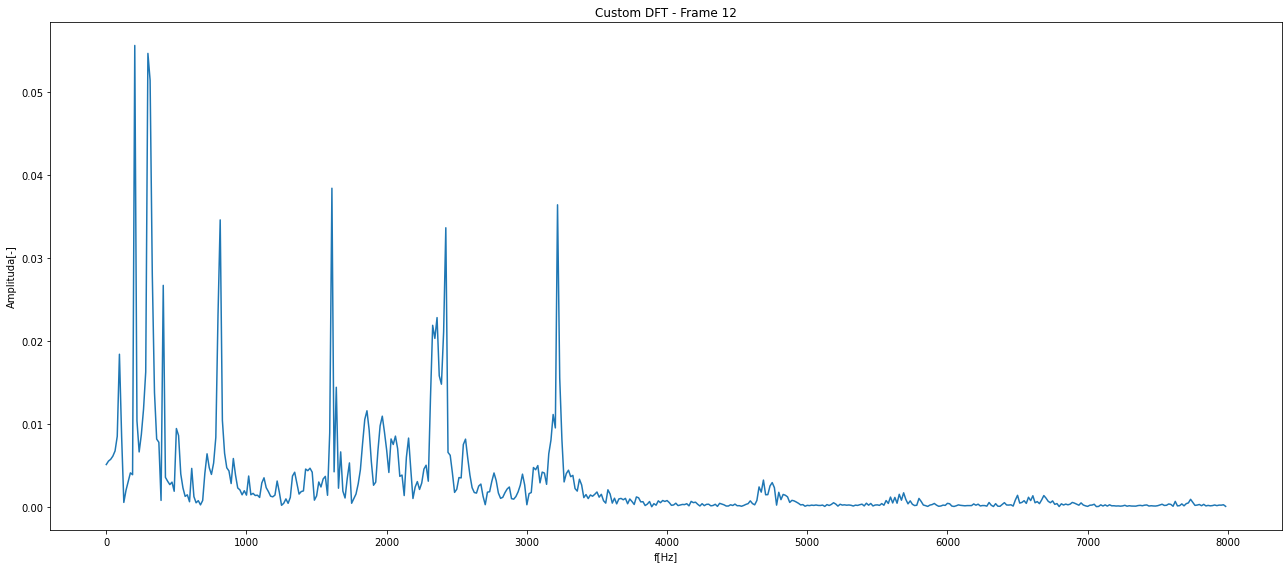
\includegraphics[scale=0.5,keepaspectratio]{Figure_5}
	\caption{Custom implementovaná funkce DFT}
\end{figure}
\end{landscape}

\begin{landscape}
\begin{figure}[H] 
	\centering
	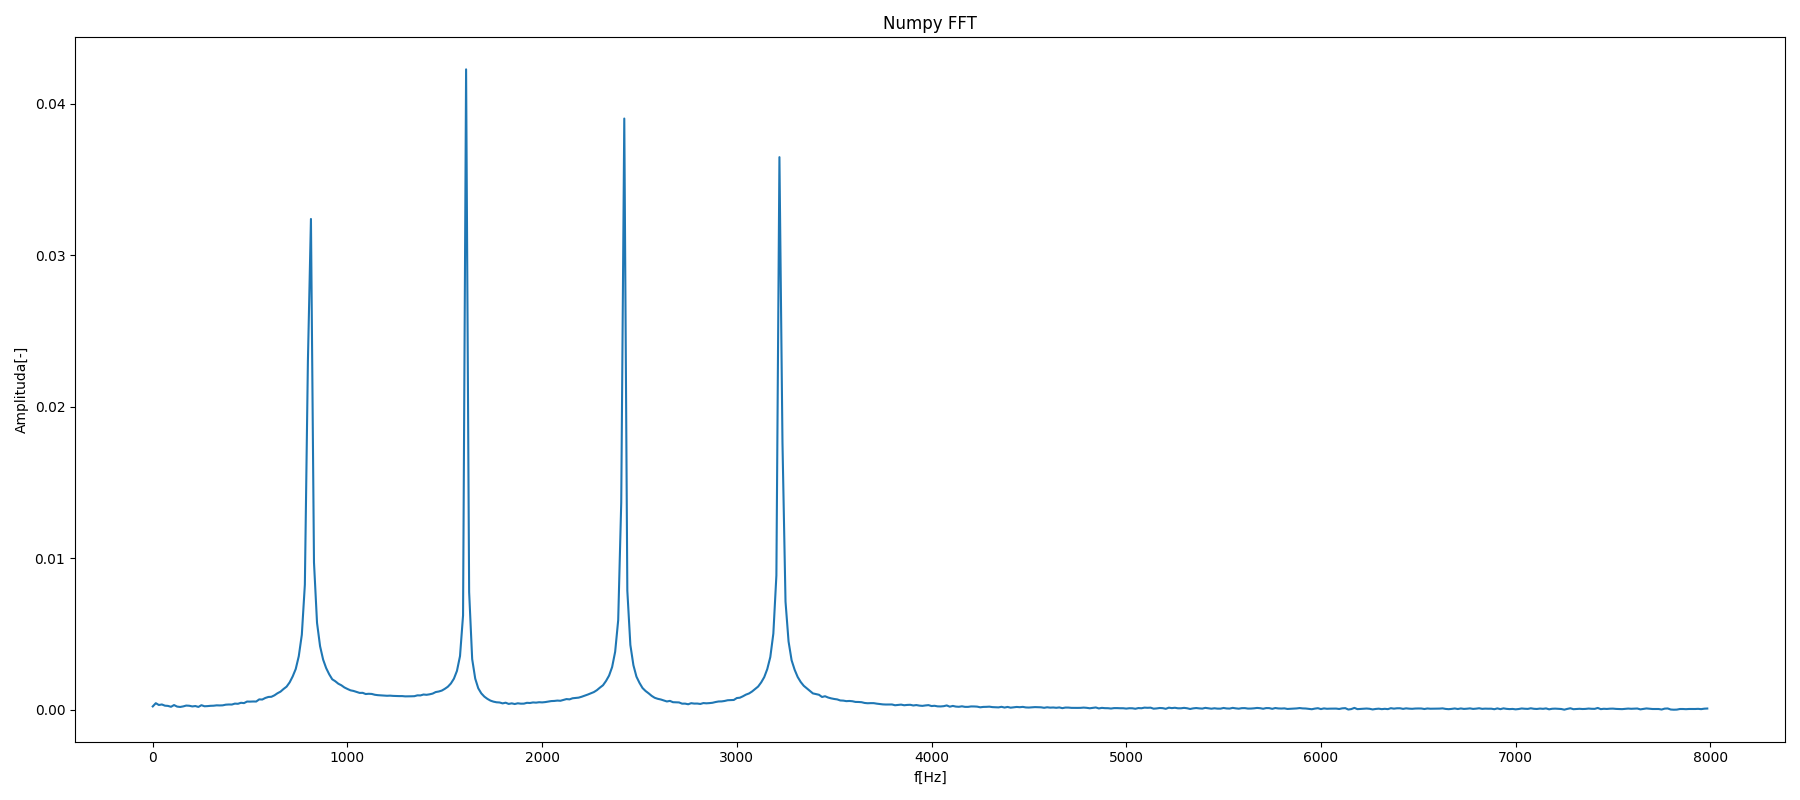
\includegraphics[scale=0.5,keepaspectratio]{Figure_4}
	\caption{Buildin FFT z knihovny numpy}
\end{figure}
\end{landscape}